\documentclass[tikz,border=2pt]{standalone}
\usepackage{amsmath}
\usepackage{pgfplots}
\pgfplotsset{compat=1.18}
\usetikzlibrary{arrows.meta}
\begin{document}
% Stationary proportions pi = (0.2, 0.16, 0.64) as widths, class premiums c = (200, 200, 100) as heights:
% the areas 40 + 32 + 64 = 136 = b(lambda), the stationary mean premium (level line of equal total area).
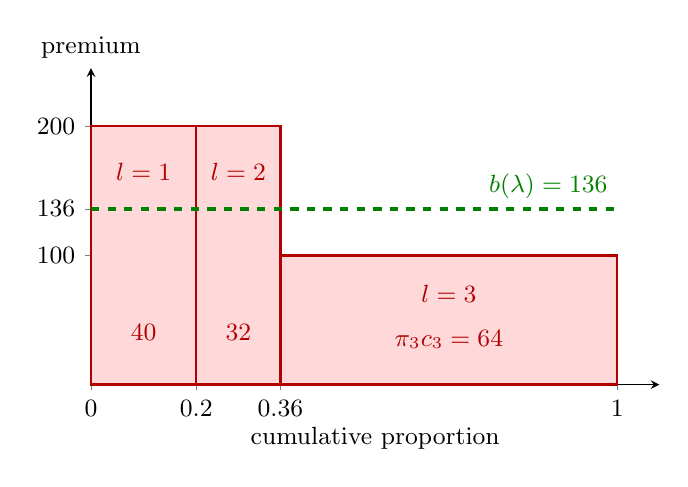
\begin{tikzpicture}[font=\small, >={Latex[length=2mm]}]
  \begin{axis}[
    axis lines=left, xmin=0, xmax=1.08, ymin=0, ymax=245,
    xtick={0,0.2,0.36,1}, ytick={100,136,200},
    xlabel={cumulative proportion}, ylabel={premium},
    xlabel style={at={(axis description cs:0.5,0)}, anchor=north, yshift=-12pt},
    ylabel style={rotate=-90, at={(axis description cs:0,1)}, anchor=south},
    width=8.8cm, height=5.6cm, clip=false
    ]
    \draw[red!70!black, thick, fill=red!15] (axis cs:0,0) rectangle (axis cs:0.2,200);
    \draw[red!70!black, thick, fill=red!15] (axis cs:0.2,0) rectangle (axis cs:0.36,200);
    \draw[red!70!black, thick, fill=red!15] (axis cs:0.36,0) rectangle (axis cs:1,100);
    \node[red!70!black] at (axis cs:0.1,165) {$l=1$};
    \node[red!70!black] at (axis cs:0.28,165) {$l=2$};
    \node[red!70!black] at (axis cs:0.68,70) {$l=3$};
    \node[red!70!black] at (axis cs:0.1,40) {$40$};
    \node[red!70!black] at (axis cs:0.28,40) {$32$};
    \node[red!70!black] at (axis cs:0.68,35) {$\pi_3c_3=64$};
    \draw[green!50!black, very thick, dashed] (axis cs:0,136) -- (axis cs:1,136);
    \node[green!50!black, anchor=south east] at (axis cs:1,136) {$b(\lambda)=136$};
  \end{axis}
\end{tikzpicture}
\end{document}
